\documentclass[conference, a4paper]{IEEEtran}

\usepackage{graphicx}
\usepackage{float}
\usepackage{xeCJK}

% --- 字型設定 ---
\setCJKmainfont{標楷體} % 中文設定為標楷體
\setmainfont{Times New Roman} % 英文設定為 Times New Roman

\usepackage{amsmath}
\usepackage{booktabs}
\usepackage{enumitem}
\setlist[itemize]{label=-}

\title{Performance Analysis of Sorting Algorithms: Insertion, Bubble, and Quick Sort in Java}

\author{\IEEEauthorblockN{蔡晟旭 (Student ID: 1113405013)}
\IEEEauthorblockA{國立澎湖科技大學 資訊工程學系 \\
National Penghu University of Science and Technology}}

\begin{document}

\maketitle

\begin{abstract}
本報告旨在實證分析三種不同複雜度等級的排序演算法：插入排序（Insertion Sort）、氣泡排序（Bubble Sort）與快速排序（Quick Sort） [cite: 255, 257, 292, 341]。透過 Java 程式環境手工實作上述演算法，並針對資料規模 $n$ 從 1,000 至 100,000 的隨機陣列進行效能測試 [cite: 340, 353]。實驗重點在於觀察 $O(n \log n)$ 演算法與多種 $O(n^2)$ 演算法在處理大規模資料時的顯著效能差異 [cite: 366]。

\vspace{0.2cm}
\textbf{GitHub Repository:} https://github.com/tch107146/Algorithm-0304-Assignments-2
\end{abstract}

\begin{IEEEkeywords}
Sorting Algorithms, Quick Sort, Bubble Sort, Insertion Sort, Big-O Notation, Java.
\end{IEEEkeywords}

\section{Introduction}
在計算機科學中，排序演算法的效率直接影響系統性能 [cite: 69, 84]。本次實驗（Assignment 2）核心目標是透過實際測量執行時間，掌握 $O(n \log n)$ 與 $O(n^2)$ 演算法在處理巨量資料時的效能鴻溝 [cite: 366]。

\section{Methodology}
本實驗實作並分析了三種排序演算法：
\begin{itemize}
    \item \textbf{Quick Sort}：採用分治法，平均時間複雜度為 $O(n \log n)$ [cite: 337, 338]。
    \item \textbf{Insertion Sort}：逐一插入元素，時間複雜度為 $O(n^2)$ [cite: 273, 274]。
    \item \textbf{Bubble Sort}：相鄰交換，時間複雜度為 $O(n^2)$ [cite: 308, 314]。
\end{itemize}

\section{Implementation Details}
本實驗採用 Java 實作，細節如下：
\begin{itemize}
    \item \textbf{Core Implementation}: 嚴格遵守不使用內建工具包之規定 [cite: 71, 87]。
    \item \textbf{Stability \& Consistency}: 針對每個級距資料量，確保比較之基準資料一致。
    \item \textbf{Time Metric}: 使用毫秒級計時擷取演算法完成排序所需時間。
\end{itemize}

\section{Experimental Results}
各演算法在不同資料規模 $n$ 下的實測數據如表 \ref{tab:results} 所示。

\begin{table}[H]
    \centering
    \caption{Sorting Performance Comparison (milliseconds)}
    \label{tab:results}
    \begin{tabular}{@{}lccc@{}}
        \toprule
        \textbf{Data Size ($n$)} & \textbf{Quick Sort} & \textbf{Insertion Sort} & \textbf{Bubble Sort} \\ \midrule
        1,000            & 0                   & 2                       & 2                    \\
        10,000           & 2                   & 18                      & 76                   \\
        50,000           & 2                   & 427                     & 2343                 \\
        100,000          & 5                   & 1698                    & 9680                 \\ \bottomrule
    \end{tabular}
\end{table}

圖 \ref{fig:screenshot} 為本次實驗之終端機執行結果截圖。

\begin{figure}[H] 
  \centering
  \IfFileExists{screenshot.png}{
    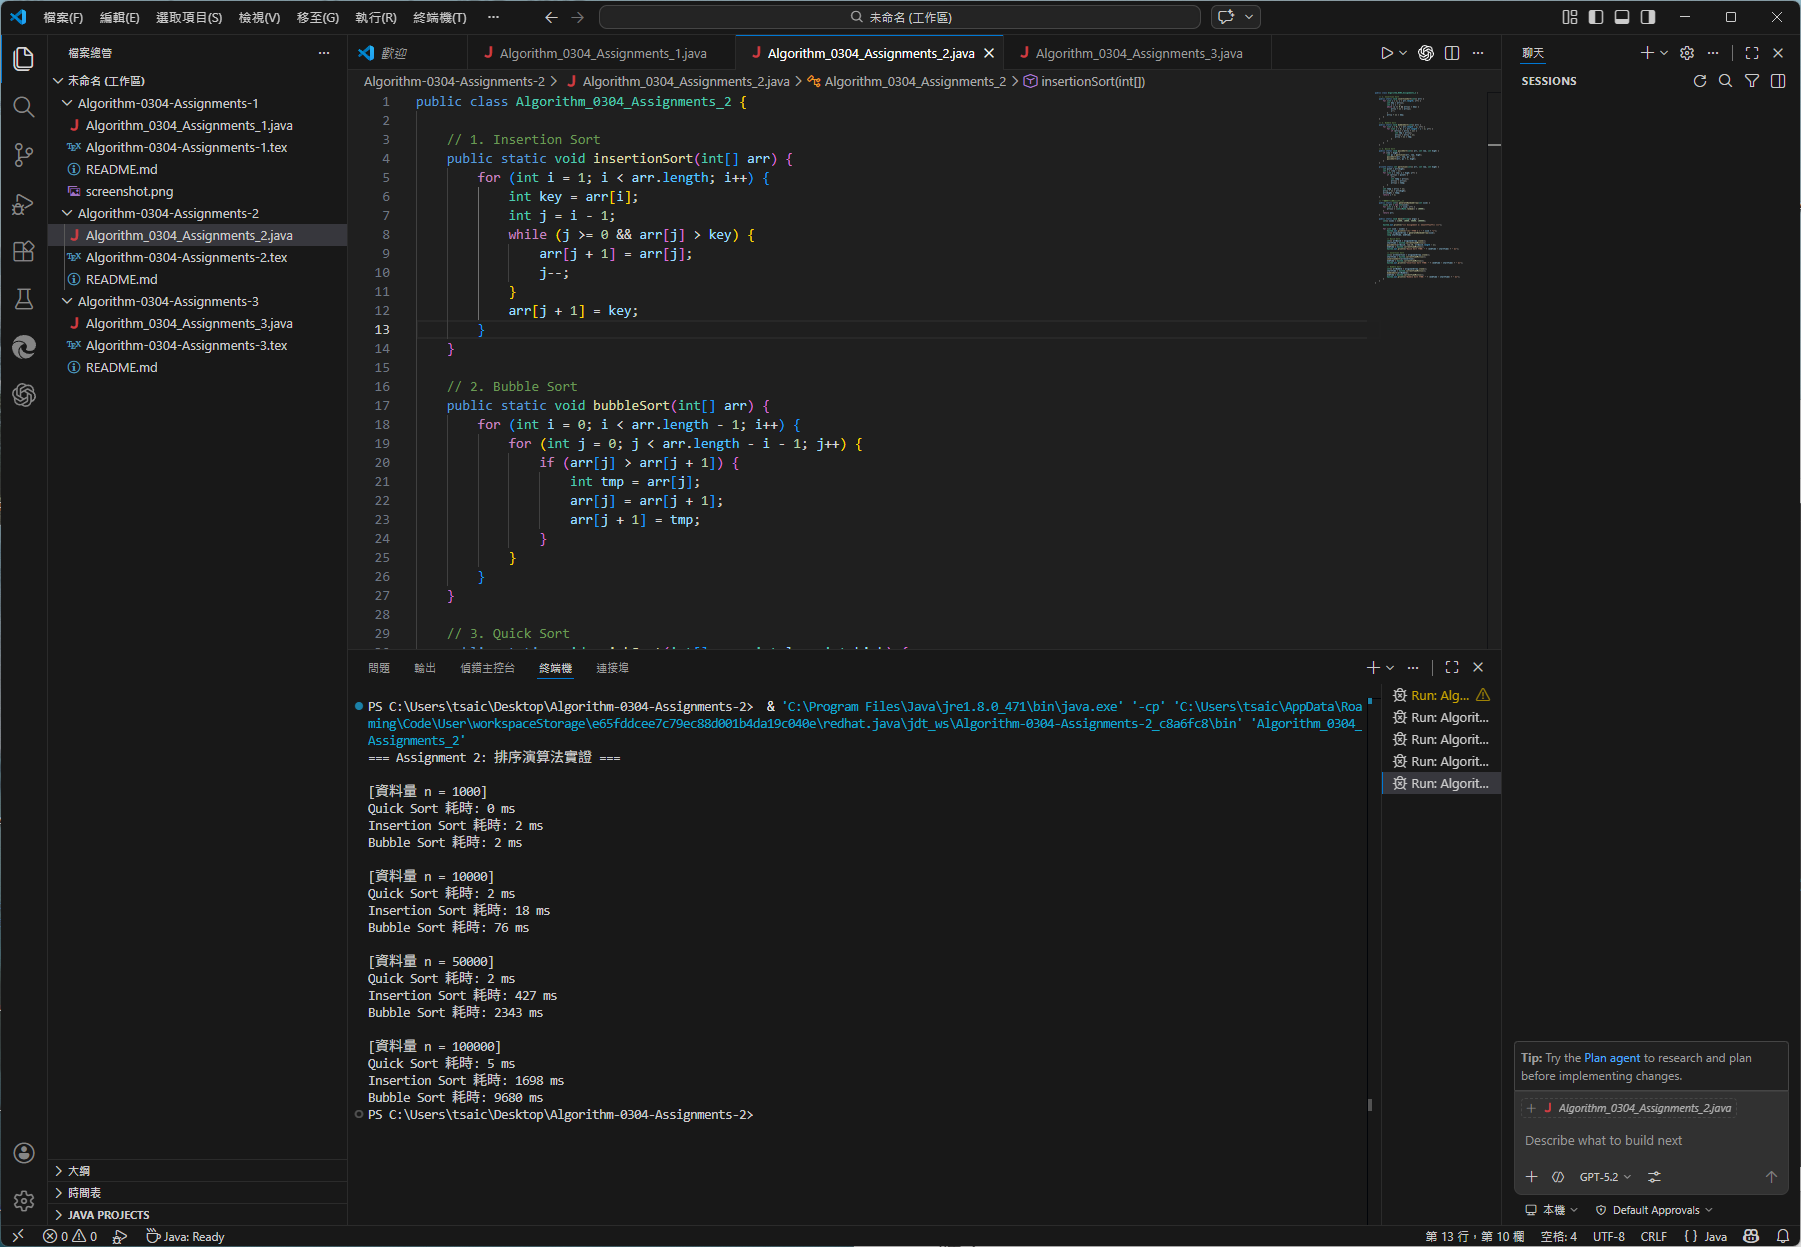
\includegraphics[width=0.9\columnwidth]{screenshot.png}
  }{
    \framebox{\parbox{0.8\columnwidth}{\centering \vspace{1.5cm} [圖片檔案 screenshot.png 缺失] \\ 請放置於同目錄 \vspace{1.5cm}}}
  }
  \caption{Terminal output for Assignment 2 execution.}
  \label{fig:screenshot}
\end{figure}

\section{Discussion}
從實測數據可觀察到：
\begin{enumerate}
    \item \textbf{Quick Sort 的穩定性}：即使資料量達 100,000，Quick Sort 僅耗時 5 ms，體現了 $O(n \log n)$ 的優異擴展性 [cite: 366]。
    \item \textbf{Bubble Sort 的代價}：在 $n=100,000$ 時，Bubble Sort 耗時高達 9680 ms，遠超 Insertion Sort。這反映了頻繁交換操作帶來的巨大常數代價 [cite: 291, 316]。
\end{enumerate}

\section{Conclusion}
本實驗實證了不同排序演算法的效能特徵 [cite: 357]。在巨量資料處理中，應優先選擇 Quick Sort 以維持系統效能 [cite: 366]。

\section{References}
\noindent [1] X.-R. Huang, \textit{Lecture 0: Preliminary Basic knowledge}, National Penghu University of Science and Technology, 2026[cite: 7, 8, 10]. \par
\noindent [2] T. H. Cormen et al., \textit{Introduction to Algorithms}, 3rd ed. MIT Press, 2009.

\end{document}